\documentclass[12pt]{article}

\usepackage[bottom = 15mm]{geometry}
\usepackage[utf8]{inputenc}
\usepackage[T2A]{fontenc}
\usepackage[russian]{babel}
\usepackage{graphicx}
\usepackage{caption}
\usepackage{amssymb, amsmath}


\textwidth = 16 cm
\textheight = 23  cm
\oddsidemargin = 0 pt
\topmargin = -1.5 cm
\parindent = 20 pt
\parskip = 0 pt
\flushbottom



\title{{\bf Задача 3.\,3.\,3 \\ Опыт Милликена}}
\author{Лось Денис (группа 611)}
\date{26 сентября 2017}




\begin{document}

\maketitle

\paragraph{Цель работы: } измерение элементарного заряда методом масляных капель.

\paragraph{В работе используются: } плоский конденсатор в защитном кожухе, измерительный микроскоп, электростатический вольтметр, электронный секундомер, переключатель напряжения, пульверизатор с маслом.

\section*{Экспериментальная установка}
Схема установки представлена на рис.1. Масло разбрызгивается пульверизатором. Капли масла попадают в конденсатор $C$ через небольшое отверствие в верхней пластине. При этом часть из них вследствие трения о воздух приобретает случайный по абсолютной величине и знаку электрический заряд.
\par
	Напряжение на пластины подаётся с регулируемого выпрямителя и измеряется вольтметром $V$. Ключ $K$ позволяет менять направления поля в конденсаторе, чтобы можно было работать как с отрицательно, так и с положительно заряженными каплями. При замыкании ключа $K$ конденсатор разряжается через дополнительное сопротивление $R \approx 10 $ МОм.
\begin{figure}[h!]
	\centering
	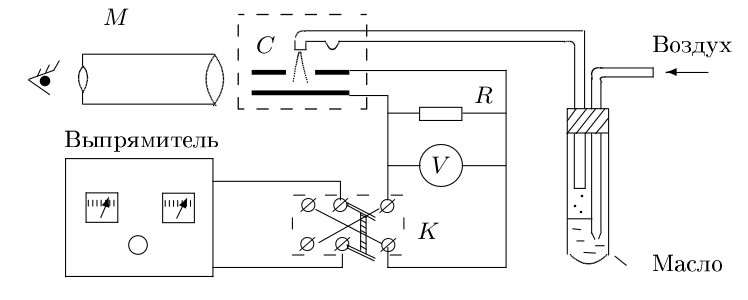
\includegraphics[width = 12cm, height = 6cm]{image1.png}
	\caption{Схема экспериментальной установки для измерения заряда электрона}	
\end{figure}	
\par
	Дискретность заряда может быть обнаружена лишь в том случае, если ошибка $\delta q$ в измерении заряда капли существенно меньше абсолютной величины заряда электрона $e$. Допустимая относительная ошибка опыта $\delta q / q$ должна быть поэтому много меньше $e / q = 1 / n$, где $n$ --- заряд капли выраженный в числе зарядов электрона. Этому условию тем легче удовлетворить, чем меньше число $n$. В нашем эксперименте трудно определить $q$ c точностью лучше $5 \%$. Заряд капли должен поэтому быть существенно меньше $20$ зарядов электрона --- лучше всего, если он не превосходит пяти электронных зарядов.
\section*{Ход работы}
\begin{enumerate}
	\item
		При дальнейших вычислениях потребуются значения некоторых величины, характеризующих данную установки: расстояние между пластинами $l = 0.725$ см, плотность масла $\rho = 0.898 \, \text{г}\, / \text{cм}^3$, коэффициент внутреннего трения воздуха $\eta = 1.83 \cdot 10^{-5}$ Па $\cdot$ с.
	\item
		В начале опыта позволим капелькам свободно падать 5 - 10 секунд при выключенном электрическом поле для того, чтобы наиболее крупные капли успели упасть на нижнюю пластину. Из оставшихся в поле зрения капель выберем одну и проведём с ней серию измерений, наблюдая её падение под действием силы тяжести и подъём под действием электрического поля, т.е. будем будем измерять время падения под действием силы тяжести $t_0$ и время подъёма под действием электрического поля $t$. 
	\item	
	 	Проделаем несколько серий таких измерений, каждый раз регистрируя величину $V$. При этом будем иметь в виду, что заряд капли может измениться во время наблюдений. Чтобы вовремя отбросить такие случаи, будем внимательно следить за движением капли и прекращать измерения, в ходе которых капля изменила скорость подъёма.	 	
		\begin{table}[h!]
			\centering
			\begin{tabular}{|c|c|c|c|c|c|c|c|c|c|c|}
 	           \hline
    	        $t_0$, c & 44.00 & 46.00 & 46.98 & 44.18 & 46.09 & 44.45 & 44.42 & 43.18	  \\
        	   \hline
      		   $t$, c & 11.73 & 11.20 & 11.69 & 12.45 & 12.26 & 11.73 & 11.25 & 12.03  \\			
			   \hline
			\end{tabular}
			\caption{Измерения для первой капли при $V = 400 $ В и $h = h_0 = 1$ мм}
		\end{table}
		\begin{table}[h!]
			\centering
			\begin{tabular}{|c|c|c|c|c|c|c|c|}
 	           \hline
    	        $t_0$, c & 24.66 & 28.26 & 30.06 & 28.34 & 28.30 & 26.50 \\
        	   \hline
      		   $t$, c & 9.97 & 10.58 & 10.33 & 9.92 & 10.34 & 9.82 \\
			   \hline
			\end{tabular}
			\caption{Измерения для второй капли при $V = 400 $ В и $h = 2h_0 = 1$ мм}
		\end{table}
		\begin{table}[h!]
			\centering
			\begin{tabular}{|c|c|c|c|c|c|}
 	           \hline
    	        $t_0$, c & 23.17 & 23.35 & 23.20 & 24.14 & 25.04 \\
        	   \hline
      		   $t$, c & 10.61& 10.66 & 10.88 & 11.15 & 10.21 \\
			   \hline
			\end{tabular}
			\caption{Измерения для третьей капли при $V = 300 $ В и $h = 2h_0 = 1$ мм}
		\end{table}
		\newpage
		\begin{table}[h!]
			\centering
			\begin{tabular}{|c|c|c|c|c|c|}
 	           \hline
    	        $t_0$, c & 24.70 & 26.62 & 23.51 & 25.38 & 26.41 \\
        	   \hline
      		   $t$, c & 29.17 & 27.86 & 29.32 & 28.06 & 29.32 \\
			   \hline
			\end{tabular}
			\caption{Измерения для четвёртой капли при $V = 300 $ В и $h = 2h_0 = 1$ мм}
		\end{table}
		\begin{table}[h!]
			\centering
			\begin{tabular}{|c|c|c|c|c|}
 	           \hline
    	        $t_0$, c & 14.71 & 16.1 & 14.20 & 14.12 \\
        	   \hline
      		   $t$, c & 19.70 & 19.95 & 19.82 & 19.74 \\
			   \hline
			\end{tabular}
			\caption{Измерения для пятой капли при $V = 500 $ В и $h = h_0 = 1$ мм}
		\end{table}
		\begin{table}[h!]
			\centering
			\begin{tabular}{|c|c|c|c|c|}
 	           \hline
    	        $t_0$, c & 19.00 & 18.19 & 18.75 & 18.37 \\
        	   \hline
      		   $t$, c & 13.99 & 13.88 & 14.30 & 13.73 \\
			   \hline
			\end{tabular}
			\caption{Измерения для шестой капли при $V = 500 $ В и $h = h_0 = 1$ мм}
		\end{table}
	\item
		Для всех исследованных капель рассчитаем среднее значение $q$, учитывая случайную погрешность.
		\[
			q = \frac{9 \pi l}{V} \sqrt{\, \frac{2 \eta^3}{\rho g}\mathstrut} \left(\frac{h}{t} + \frac{h_0}{t_0} \right) \left(\frac{h_0}{t_0}\right)^{\frac{1}{2}}
		\]	
		 \begin{table}[h!]
		 	\centering
		 	\begin{tabular}{|c|c|c|}
		 	\hline
		 	$N_\text{капли}$ & $q$ , $10^{-10}$ ед. СГСЭ & $\sigma_q \, \% $ \\
		 	\hline
		 	1 & 9.179 & 3.2\\
		 	2 & 9.012 & 6.3 \\
		 	3 & 12.712 & 5.6\\
		 	4 & 5.874 & 3.9\\
		 	5 & 14.153 & 6.5\\
		 	6 & 13.359 & 2.5\\
		 	\hline
		 	\end{tabular}
		 \end{table}
	\item
		Для определения наибольшего общего делителя зарядов, который в случае успешности эксперимента будет равен $e$, построим график $q = \alpha k$, где $k$ --- порядковый номер заряда в неубывающем ряду, построенному по таблице. Учитывая случайную погрешность для зарядов, будем считать, что заряды третьей, пятой и шестой капель, а также первой и второй равны, поэтому в неубывающий ряд значений поставим только их среднее. По наклону прямой, найденному с помощью метода наименьших квадратов, получим величину элементарного заряда.
   	\begin{align*}
		e &= \left(4.6 \pm 0.3 \right) \cdot 10^{-10} \, \text{ед. СГСЭ} \quad \left(\sigma_q = 5.5 \% \right) \\
		e &= \left(1.53 \pm 0.08 \right)  \cdot 10^{-19} \, \text{Кл} 
	\end{align*}	
	\newpage	
	\begin{figure}[h!]
		\centering
		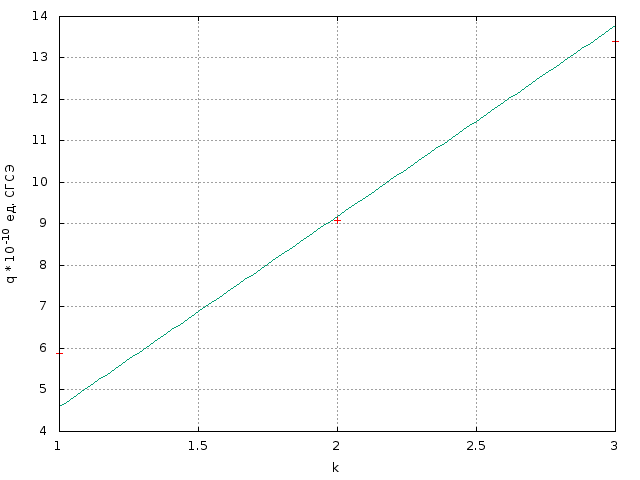
\includegraphics[width = 12cm, height = 6.5cm]{plot1.png}
		\caption{График зависимости $q = \alpha k$}
	\end{figure}
   \item
   		Оценим время релаксации $\tau = v_\text{уст} / g$ и расстояние $s$, которое прошла бы капля за этом время с установшейся скоростью по результатам первого измерения для первой капли.
   		\begin{align*}
   			\tau &= \frac{h_0}{g t_0} = 2.3 \, \text{мкс} \\
   			s &= \frac{1}{g}\, \left(\frac{h_0}{t_0}\right)^2 = 5.3 \cdot 10^{-8} \, \text{мм} \ll 1 \, \text{мм}
   		\end{align*}
   	\item
   		Для оценки точности измерений подвесим одну из капель в электрическом поле. Определим соответствующее напряжение, затем отключим его и измерим время падения капли на расстояние трёх делений шкалы. Поменяв полярность напряжения, вернём каплю на прежнее место. Повторим данную процедуру несколько раз. Отсюда оценим заряд капли по приведённой формуле (т.е считая $t = \infty$), а также оценим точность измерения заряда этой капли.
   		\[
   			q = 9 \pi \sqrt{\frac{2 \eta^3 h^3}{g \rho}} \cdot \frac{l}{V t_0^{3/2}}
   		\]
   		\begin{table}[h!]
   			\centering
   			\begin{tabular}{|c|c|c|}
   			\hline
   			$V$, В & $t$, c & $q$, $10^{-10}$ ед. СГСЭ \\
   			\hline
   			800 & 7.43 & 9.200\\
   			\hline
   			700 & 6.99 & 11.523\\
   			\hline
   			750 & 7.42 & 9.834\\
   			\hline
   			700 & 7.31 & 10.775\\
   			\hline
   			720 & 7.25 & 10.606\\
   			\hline
   			\end{tabular}
   		\end{table}	
		\[
			q = \left(10.4 \pm 0.09 \right) \cdot 10^{-10} \, \text{ед. СГСЭ} \quad \left(\sigma_q = 8.6 \%\right)
		\]	   		
   		
\end{enumerate}	
	
\end{document}